\documentclass[10pt, handout, envcountsect]{beamer} % text size parameter 10, ratio parameter, handout (in case of need to share)

\usetheme{Madrid} % view themes and colors at https://www.overleaf.com/learn/latex/Beamer#Reference_guide
% \usecolortheme{seahorse}

% \usepackage{pgfpages} % handouts (in case of need to share)
% \pgfpagesuselayout{4 on 1}[a4paper, border shrink=5mm]

\setbeamertemplate{navigation symbols}{} % hides navigation buttons at buttom 
%\setbeamertemplate{footline}[frame number]{} % gets rid of bottom navigation bars
\setbeamercovered{transparent} % makes transparent paramters

\setbeamertemplate{headline}{} % hides navigation bar on top

\usepackage{graphicx} % Required for inserting images
\title[Paper Review]{Paper Review}
\subtitle{
\large{Bayesian neural networks become heavier-tailed with depth}
\\
\vspace{3pt}
\normalsize{Mariia Vladimirova, Julyan Arbel, Pablo Mesejo}
}
\author{Marat Khusainov}
\date{September 2023}

\begin{document}

\maketitle

% ------------------------------

\begin{frame}{Outline}

\tableofcontents

\end{frame}

\section{Motivation $\&$ Problem statement}
% ------------------------------

\begin{frame}{Motivation $\&$ Problem statement}
\begin{itemize}
    \item What are hidden units prior distributions in Bayesian neural networks under assumption of independent Gaussian weights?
\end{itemize}

$$
\boldsymbol{g}^{(\ell)}(\boldsymbol{x})=\boldsymbol{W}^{(\ell)} \boldsymbol{h}^{(\ell-1)}(\boldsymbol{x}), \quad \boldsymbol{h}^{(\ell)}(\boldsymbol{x})=\phi\left(\boldsymbol{g}^{(\ell)}(\boldsymbol{x})\right).
$$

\begin{figure}[h]
    \centering
    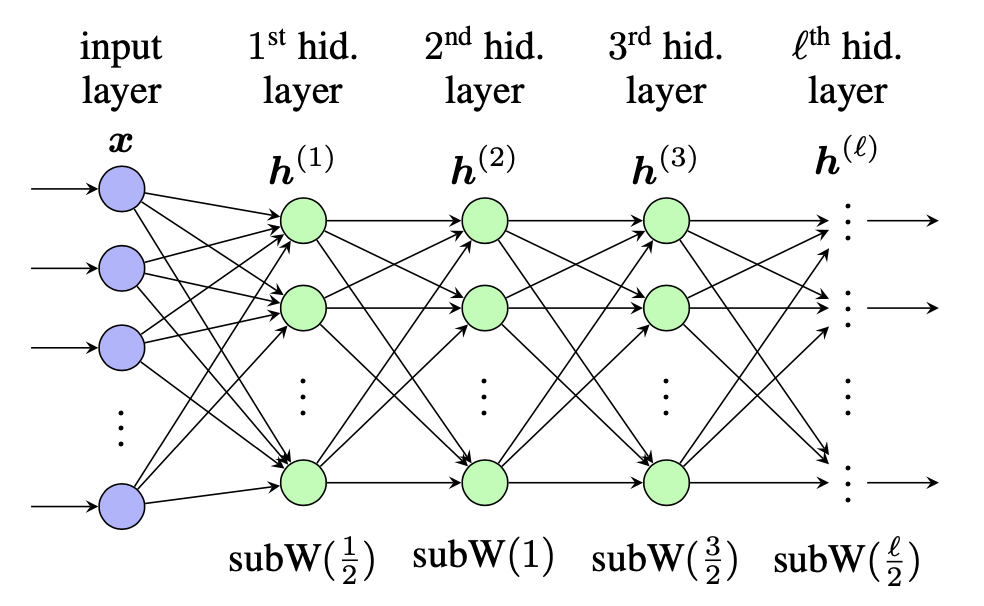
\includegraphics[width=7.5cm,]{figure_2.png}
    \caption{Neural network architecture and characterization of the $\ell$-layer units prior distribution as sub-Weibull distribution with tail parameter $\ell/2$.}
    % \label{}
\end{figure} 
    
\end{frame}


\section{Theory}
% ------------------------------
\begin{frame}{Definitions $\&$ Assumption on neural network}

\begin{definition}[Sub-Weibull random variable]
A random variable $X$, that satisfies
$$
\mathbb{P}(|X| \geq x) \leq \exp \left(-x^{1 / \theta} / K\right) \quad \text { for all } x \geq 0 .
$$
for $K>0$, is called a sub-Weibull random variable with the tail parameter $\theta>0$, which is denoted by $X \sim \operatorname{subW}(\theta)$.

\end{definition}

Let all weights (including biases) be independent and have zero-mean normal distribution
$
W_{i, j}^{(\ell)} \sim \mathcal{N}\left(0, \sigma_w^2\right),
$
for all $1 \leq \ell \leq L, 1 \leq i \leq H_{\ell-1}$ and $1 \leq j \leq H_{\ell}$.

\begin{definition}[Extended envelope property for nonlinearities]
A nonlinearity $\phi: \mathbb{R} \rightarrow \mathbb{R}$ is said to obey the extended envelope property if there exist $c_1, c_2, d_1, d_2 \geq 0$ such that the following inequalities hold
$$
\begin{aligned}
& |\phi(u)| \geq c_1+d_1|u| \quad \text { for all } u \in \mathbb{R}_{+} \text {or } u \in \mathbb{R}_{-}, \\
& |\phi(u)| \leq c_2+d_2|u| \quad \text { for all } u \in \mathbb{R} .
\end{aligned}
$$

\end{definition}
    
\end{frame}

% ------------------------------

\begin{frame}{Main theorem}

% \begin{lemma}
% Let a nonlinearity $\phi: \mathbb{R} \rightarrow \mathbb{R}$ obey the extended envelope property. Then for any symmetric random variable $X$ the following asymptotic equivalence ${ }^3$ holds
% $$
% \mathbb{E}\left[\phi(X)^k\right] \asymp \mathbb{E}\left[X^k\right], \quad \text { for } k \rightarrow \infty .
% $$
% \end{lemma}

\begin{theorem}[Sub-Weibull units]
Consider a feed-forward Bayesian neural network with Gaussian priors with nonlinearity $\phi$ satisfying the extended envelope condition. Then conditional on the input $\boldsymbol{x}$, the marginal prior distribution induced by forward propagation on any unit (pre- or post-nonlinearity) of the $\ell$-th hidden layer is sub-Weibull with optimal tail parameter $\theta=\ell / 2$. That is for any $1 \leq \ell \leq L$, and for any $1 \leq m \leq H_{\ell}$,
$$
U_m^{(\ell)} \sim \operatorname{subW}(\ell / 2)
$$
where $U_m^{(\ell)}$ is either a pre-nonlinearity $g_m^{(\ell)}$ or a post-nonlinearity $h_m^{(\ell)}$.
    
\end{theorem}
    
\end{frame}

\section{Experiment}
% ------------------------------
\begin{frame}{Experiment}

% These densities are obtained as kernel density estimators from a sample of size 105 from the prior on the pre-nonlinearities, which is itself obtained by sampling 105 sets of weights W from the Gaussian prior (2) and forward propagation via (1). The three hidden layers of neural network have H1 = 25, H2 = 24 and H3 = 4 hidden units, respectively. Being a linear combination involving symmetric weights W , pre-nonlinearities g are also symmetric, thus we visualize only their positive part. The input vector x ∈ R50 is sampled 

Densities are obtained as kernel density estimators from a sample of size $10^5$ from the prior on the pre-nonlinearities, which is itself obtained by sampling $10^5$ sets of weights $\boldsymbol{W}$ from the Gaussian prior and forward propagation.

\vspace{3pt}

\begin{itemize}
    % \item Densities are obtained as kernel density estimators from a sample of size $10^5$ from the prior on the pre-nonlinearities, which is itself obtained by sampling $10^5$ sets of weights $\boldsymbol{W}$ from the Gaussian prior and forward propagation
    \item 3 hidden layers of NN have $H_1 = 25, H_2 = 24$ and $H_3 = 4$ hidden units
    \item The nonlinearity $\phi$ is the ReLU function
    \item $\boldsymbol{x} \in \mathbb{R}^{50}$ is sampled from a standard normal distribution.
\end{itemize}

\begin{figure}[h]
    \centering
    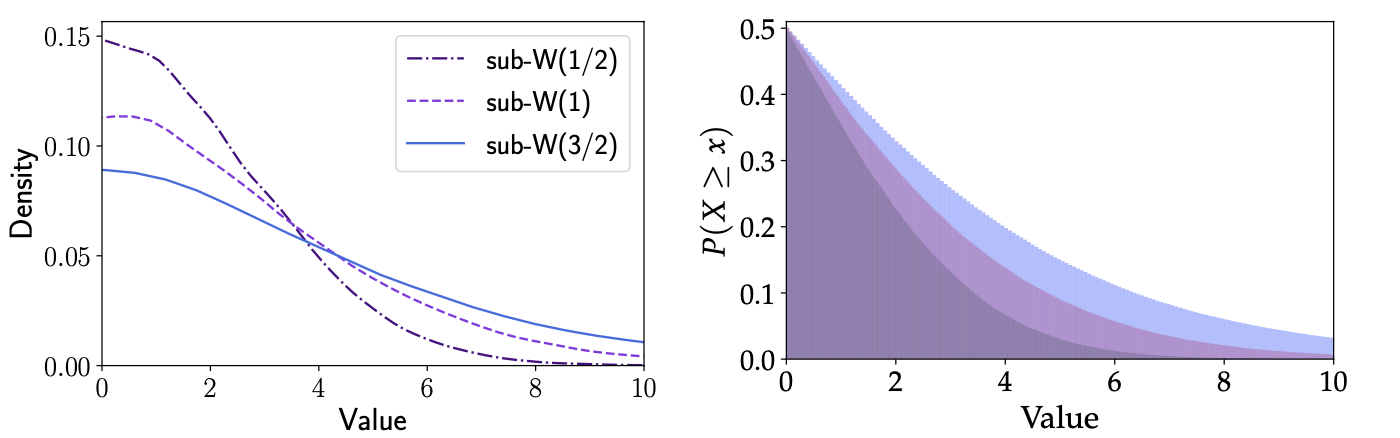
\includegraphics[width=12cm,]{figure_1.png}
    \caption{Illustration of the first three layers hidden units marginal prior distributions.}
    % \label{}
\end{figure} 
    
\end{frame}

% ------------------------------


\end{document}

